\chapter{Estudos de Caso}

Neste capítulo, apresentaremos os estudos que estão em andamento ao colaborarmos com a plataforma livre Noosfero (cujo processo de desenvolvimento foi descrito na seção~\ref{sec:dev-noosfero}), explicitando alguns resultados iniciais, desta primeira fase do trabalho.

O estudo deste trabalho, nesta primeira fase, foi baseado nos seguintes ambientes de
rede social que utilizam a plataforma noosfero:
%
o portal Participa.Br\footnote{Participa.Br}, para as observações sobre a usabilidade do Noosfero;
%
a rede Comunidade.UnB\footnote{comunidade.unb.br} e o Portal UnB Gama\footnote{fga.unb.br}, para as observações sobre os testes automatizados no Noosfero;
%

O Portal da participação Social (Participa.Br) é um portal que agrega informações sobre oportunidades de participação social no governo federal e estimula a formação de comunidades em torno de temas ligados à participação.
%
Informa sobre as consultas públicas, oferece ambientes para interação em vídeo e chat em eventos de governo. É um repositório das metodologias das conferências de políticas públicas. O Participa.Br capta demandas da sociedade que não passem, necessariamente, pelos fluxos formais de participação. É uma plataforma para ampliar o debate entre a sociedade civil e o governo.

A rede Comunidade UnB, que se encontra em ambiente de testes, porém disponível para acesso externo, é uma instância do Noosfero instalada através de um pacote em um servidor do Centro de Difusão de Tecnologia e Conhecimento (CDTC)\footnote{\url{cdtc.org.br}} da UnB. O propósito da rede Comunidade UnB é tornar-se um ambiente de colaboração entre os alunos da Universidade de Brasília, tanto de graduação quanto de pós-graduação, possibilitando criação comunidades e blogs para discussões, ou a disponibilização de artigos, trabalhos de graduação e pós-graduação onde qualquer membro da universidade tenha acesso.

O Portal UnB Gama é um portal utilizado pela Faculdade do Gama da UnB para publicações de notícias sobre a própria faculdade, realização de eventos e divulgação de palestras.

\section {Estudo sobre Usabilidade: Participa.Br}

\begin{comment}
%\subsection{Justificativa}		
%TODO: No TCC 2, pensar em colocar esta parte na introdução/problema.

No ano 2000 foi criado o programa de Governo Eletrônico (e-GOV) \footnote{\url{governoeletronico.gov.br}} que têm como principais objetivos democratizar o acesso a informação e dinamizar a prestação de serviços públicos eletrônicos com foco em eficiência e efetividade das funções governamentais prestadas ao cidadão.
%
O Governo Federal adotou várias práticas de padrões para melhorar o acesso e a divulgação das informações e dos serviços do governo eletrônico, respeitando as particularidades de cada cidadão. Por isso foi criado o Modelo de Acessibilidade do Governo Federal (e-MAG) \footnote{e-MAG: Cartilha de acessibilidade do governo eletrônico} que contém um conjunto de recomendações para tornar os sítios e portais acessíveis para uma maior quantidade de pessoas possíveis. 

O objetivo era de estabelecer padrões de qualidade de uso, desenho, arquitetura da informação e navegação, desenvolvimento e manutenção na gestão dos sítios governamentais. O e-PWG \footnote{e-PWG: Padrões web para o governo eletrônico}, como ficou conhecido, são padrões web para o Governo eletrônico.
%
Foi feita uma análise do sítio Participa.Br em parceria com o Instituto Federal do Rio Grande do Sul (IFRS) onde foi criado um relatório para orientar e sugerir correções que facilitarão o acesso ao seu conteúdo quanto as recomendações sobre o Modelo de Acessibilidade em Governo Eletrônico (e-MAG) e com os Padrões Web em governo Eletrônico (e-PWG). Essas recomendações buscam levantar problemas que impactarão na experiência de uso do portal pelo cidadão.
%
A ideia de fazer esse estudo experimental era de conhecer e aplicar as técnicas existentes na engenharia de usabilidade em um contexto real de uso para verificar como funcionam as técnicas utilizadas na engenharia de usabilidade para avaliação de um web-site.
%
Como já existia um estudo referente sobre a acessibilidade do portal Participa.Br, o nosso estudo se deu em avaliar a qualidade em uso do portal no sentido de verificar a satisfação dos usuários ao utilizar o portal.
%
Primeiramente foi preciso realizar um \textit{checklist} de usabilidade para verificar os possíveis problemas no portal antes de realizar os testes com os usuários. Foi utilizado as heurísticas de Nielsen para identificação dos problemas de usabilidade.

\end{comment}

O Objetivo Global deste estudo de usabilidade é analisar a interação dos usuários com o portal Participa.Br a fim de avaliar a qualidade em uso do portal. 
%
O Objetivos de Medição são (1) conhecer quem são os usuários do Participa.Br
(2) verificar problemas de usabilidade no Participa.Br;
(3) avaliar de forma subjetiva o grau de satisfação dos usuários com a utilização do portal Participa.Br. 
%
O objetivo deste estudo em si é
\textbf{analisar} o Participa.Br,
\textbf{com propósito de} avaliar qualidade em uso (ISO/IEC 9126-4),
\textbf{com respeito à} satisfação do usuário,
\textbf{do ponto de vista de} usuário,
\textbf{no contexto de} portais governamentais.

A partir dos objetivos de medição estabelecidos, foram definidas questões sobre o que é preciso saber de forma a apoiá-la a entender se o objetivo específico foi alcançado. Assim, para cada questão foram definidas as métricas relacionadas na Tabela~\ref{tabela-questoes}: 

\begin{table}[h]
\begin{tabular}{|l|l|l|}
\hline
\textbf{Questões}  & Métricas    & \begin{tabular}[c]{@{}l@{}}Diretrizes para \\ interpretação \end{tabular}  \\ \hline
\begin{tabular}[c]{@{}l@{}} Q1. Qual o perfil do usuário \\ que utiliza o  Participa.Br?  \end{tabular} &                Perfil               & \begin{tabular}[c]{@{}l@{}} Análise de Dados Estatísticos,\\ criação de personas, análise \\ dos dados qualitativos. \end{tabular}\\ \hline
\begin{tabular}[c]{@{	}l@{}} Q2. Qual o grau de satisfação\\ do usuário que utiliza o  \\ Participa.Br \end{tabular} &  \begin{tabular}[c]{@{}l@{}} Grau de satisfação \\ do usuário \end{tabular} & \begin{tabular}[c]{@{}l@{}} Escore da satisfação global\\ pelo usuário (OVERALL)   \end{tabular}                               \\ \hline
\begin{tabular}[c]{@{}l@{}} Q3. Quantidade de tempo gasto \\ para realizar as tarefas   \end{tabular}   &            Duração                   & Tempo gasto                       \\ \hline
\end{tabular}
\caption{Questões de Pesquisa}
\label{tabela-questoes}
\end{table}

Foram levantadas algumas hipóteses para este estudo experimental no Participa.Br:
\begin{enumerate}
\item A média do grau de satisfação dos usuários que já utilizaram o portal seria maior do que quem nunca utilizou?

\item O grau de satisfação dos usuários que já tinha contato com o portal é diferente dos que nunca tiveram acesso?
\end{enumerate}
% Obs: Definir melhor as hipóteses

Estas hipóteses foram criadas inicialmente pensando em verificar a diferença na satisfação entre um usuário que já utilizou o portal com um usuário que nunca utilizou.
%
Em relação a seleção dos indivíduos na primeira fase do experimento serão escolhidos pessoas com diferentes perfis que trabalham na Presidência da República e que já utilizaram o Participa.Br. Na segunda fase seriam escolhidas pessoas que nunca utilizaram o portal.

\subsection{Metodologia}

Do ponto de vista de metodológico, elencamos algumas técnicas para identificamos o perfil dos usuários do Participa.Br:

\begin{enumerate}
\item \textbf{Dados Estatísticos} (\textit{Google analytcs}, Piwiki, entre outros): Através dos dados estatísticos é possível identificar algumas informações sobre o perfil dos usuários que acessam o portal. Nas pesquisas quantitativas não são necessários o contato direto com o usuário. Esses dados estatísticos podem ser coletados de base de dados, redes sociais ou sistemas de análises de sites.

\item \textbf{Questionário de identificação de perfil dos usuários:} Para identificar o perfil dos usuários do Portal da Participação social é necessário realizar uma pesquisa qualitativa para levantamento das principais características contextuais dos usuários típicos, de modo a compreender quem são, qual o conhecimento e experiência com a internet e como utilizam para realizar seu trabalho acadêmico ou profissional. A realização dessa pesquisa será feita com os usuários do Portal da Participação Social.
%
A análise do questionário servirá para entender o perfil dos usuários do Portal da participação social, através da investigação de seus interesses. Foi levantado também algumas questões referentes ao uso das funcionalidades do Participa.Br.

\item \textbf{Identificação de Personas:} Para a definição de usuários podemos utilizar a técnica de “Persona” que são personagens fictícios criados com base em dados reais. Os Personas atuam como representantes dos usuários reais e representam as necessidades de um grupo maior. 
%
A utilização de Personas permite ter um maior foco no usuário, deixando o projeto centrado no usuário. É utilizado para a identificação de requisitos, criação de cenários e \textit{user stories}. 
%
%Para podermos identificar os personas primeiramente temos que realizar uma pesquisa quantitativa no qual podemos identificar os grupos de usuários. Após a identificação dos grupos de usuários é realizado a pesquisa qualitativa (entrevistas, coleta de dados) na qual podemos identificar as necessidades dos usuários de um determinado portal.
%
%Para criação do persona será necessário realizar entrevista com 3 pessoas de cada grupo alvo (universitários, ativistas políticos, servidores públicos, etc).

\end{enumerate}

As medidas de usabilidade neste estudo foram obtidas considerando-se três fatores: eficácia, eficiência e satisfação de uso.
%
Adotamos como paradigma de avaliação o teste de usabilidade, que consiste em avaliar o desempenho dos usuários na execução de tarefas cuidadosamente preparadas, dentro do escopo do sistema. Esse desempenho pode ser avaliado nos quesitos: número de erros e tempo de execução da tarefa. %Com essa avaliação será coletado tantos dados subjetivos em um cenário real como dados objetivos. Os dados subjetivos serão coletados através de opiniões dos participantes, comentários em relação ao uso do portal da participação social. 
Os dados obtidos consistem em medidas de tempo e desempenho dos participantes.

Elencamos algumas técnicas para avaliar a usabilidade do portal Participa.Br:

\begin{table}[h]
\begin{tabular}{|l| p{10cm} |}
\hline
Técnica & Descrição \\ \hline
Observar Usuários & Um observador irá registrar o tempo 
gasto por cada participante para concluir o estudo de caso, 
avaliar a ferramenta e se necessitou de alguma ajuda    \\ \hline
Perguntar aos usuários & Os questionários ASQ e PSSUQ 
de satisfação dos usuários será utilizado 
para coletar as opiniões dos participantes.\\ \hline
\end{tabular}
\caption{Técnicas de avaliação para os testes com usuários}
\end{table}


Segundo as pesquisas realizadas no capítulo 4 sobre técnicas de avaliações de usabilidade, é importante que antes que execute um teste de usabilidade seja feito uma avaliação da usabilidade por parte de especialistas de usabilidade.
%TODO: quais pesquisas realizadas?
%
Através das Heurísticas de Usabilidade de Nielsen e das listas de verificação,são verificados os problemas inerentes ao Participa.Br.

Levantamos algumas tarefas/cenários que devem ser executadas para a realização do teste de usabilidade com o objetivo de medir a satisfação relativa a cada tarefa. As tarefas foram pensadas levando em consideração as necessidades dos usuários do Participa.Br. Tarefas que os usuários-alvo executariam mais frequentemente e tarefas que poderiam apresentar problemas para a compreensão e execução do usuário. 

Os instrumentos de coletas de informações utilizados são dois questionários que são amplamente utilizados para medir a satisfação do usuário com produtos interativos e fornecem medidas padronizadas.
%
São eles o \textit{After-Scenario Questionnaire} (ASQ) \footnote{ASQ: Proposto por Lewis} e o \textit{Post-Study System Usabiliy Questionnaire} (PSSUQ). 
%
O ASQ é destinado ao uso em testes de usabilidade baseados em cenários. Possui três itens que abordam os seguintes componentes de usabilidade: (1) facilidade de conclusão da tarefa, (2) tempo necessário para completar uma tarefa e,(3) a adequação das instruções ou materiais de apoio fornecidos.
%
O PSSUQ é aplicado após a conclusão de todos os cenários com o propósito de fornecer uma avaliação geral geral da usabilidade do sistema. pois permite uma avaliação de usabilidade mais ampla, podendo avaliar 4 fatores e usabilidade (satisfação geral, utilidade do sistema, qualidade da interface e qualidade da informação). 

Em suma, o objetivo do teste de usabilidade é exibir os problemas de usabilidade por meio da voz dos usuários típicos. Como cada um dos usuários participantes do teste se comporta na realização das atividades.


\subsection{Variáveis}
 
a. Independentes

Foram identificadas as seguintes variáveis independentes: 

\begin{itemize}
	\item A interface do Portal da Participação Social
	\item Os cenários/tarefas para realização
	\item Perfil do usuário
	\item Contexto da avaliação
\end{itemize}

b. Dependentes


\begin{table}[h]
\begin{tabular}{|l|l|l|l|l|l|l|l|}
\hline
\textbf{Nome} & \textbf{Abreviação}  & \textbf{Entidade} & \textbf{\begin{tabular}[c]{@{}l@{}}Faixa \\ de Contagem\end{tabular}} & \textbf{\begin{tabular}[c]{@{}l@{}}Regra de \\ contagem\end{tabular}}                                                                 \\ \hline
\begin{tabular}[c]{@{}l@{}}Grau de \\ Satisfação \\ do Usuário\end{tabular}   & OVERALL                     & Satisfação                                                                                                                                                                               & \begin{tabular}[c]{@{}l@{}}Discordo \\Fortemente /\\ Concordo \\Fortemente\end{tabular} & \begin{tabular}[c]{@{}l@{}}Avalia os \\ itens 1 até 19.\end{tabular}                                \\ \hline
\begin{tabular}[c]{@{}l@{}}Grau de \\ Utilidade \\ do sistema\end{tabular}    & SYSUSE                       & Utilidade                                                                                                                                                                                & \begin{tabular}[c]{@{}l@{}}Discordo\\ Fortemente /\\ Concordo \\Fortemente\end{tabular} & \begin{tabular}[c]{@{}l@{}}Avalia os \\ itens 1 até 8.\end{tabular}                                 \\ \hline
\begin{tabular}[c]{@{}l@{}}Grau de \\ Qualidade \\ da Informação\end{tabular} & INFOQUAL                    & \begin{tabular}[c]{@{}l@{}}Qualidade \\ da Informação\end{tabular}                                                                                                                        & \begin{tabular}[c]{@{}l@{}}Discordo \\Fortemente /\\ Concordo \\Fortemente\end{tabular} & \begin{tabular}[c]{@{}l@{}}Avalia os\\ itens 9 até 15.\end{tabular}                                 \\ \hline
\begin{tabular}[c]{@{}l@{}}Grau de \\ Qualidade \\ da Interface\end{tabular}  & INTERQUAL                    & \begin{tabular}[c]{@{}l@{}}Qualidade \\ da Interface\end{tabular}                                                                                                                        & \begin{tabular}[c]{@{}l@{}}Discordo \\ Fortemente /\\ Concordo\\ Fortemente\end{tabular} & \begin{tabular}[c]{@{}l@{}}Avalia os \\ itens 16 até 18.\end{tabular}                               \\ \hline
\begin{tabular}[c]{@{}l@{}}Tempo de \\ duração de \\ uma tarefa\end{tabular}  & Tempo               &                                                                                                                               Hora*                                                              & Minutos                                                                             & Cronometro                                                                                          \\ \hline
\begin{tabular}[c]{@{}l@{}}Taxa de \\ conclusão \\ da tarefa\end{tabular}     & Conclusão                   & Conclusão                                                                                                                                                                            & 0 a 100 \%                                                                          & \begin{tabular}[c]{@{}l@{}}(Tarefas não \\ concluídas/\\ tarefas \\ concluídas)\\ *100\end{tabular} \\ \hline
\end{tabular}
\caption {Tabela de variáveis dependentes}
\end{table}

\newpage

\subsection{Recursos}

\begin{itemize}
\item Estação de trabalho para cada participante.
\item Navegador de Internet.
\item Questionário para a avaliação da usabilidade.
\item Software de Vídeo (Camtasia - versão trial) ou outro.
\end{itemize}



\subsection{Validade dos Resultados}


\begin{table}[!h]
\begin{tabular}{|p{5cm} |l|l|l|}
\hline
\textbf{Ameaça}                                                                                                                                                      & \textbf{Tipo} & Descrição da ameaça                                                                                                                                             & Tratamento                                                                                                                   \\ \hline
\begin{tabular}[c]{@{}l@{}}O esforço por pessoas \\que já conhecem o portal\\ poderá ser maior do que com \\ pessoas que nunca teve \\ contato com o portal.\end{tabular} & Externa       & \begin{tabular}[c]{@{}l@{}}Participantes que já \\ tenha conhecimento do \\ portal terá uma maior \\facilidade de uso \\ pois já conhecem \\ a ferramenta.\end{tabular} & \begin{tabular}[c]{@{}l@{}}Realizar também a \\ pesquisa com pessoas \\ que nunca tiveram \\ contato com o portal.\end{tabular} \\ \hline
Questionário não preenchido    & Conclusão     & \begin{tabular}[c]{@{}l@{}}Participantes não\\ preencherem todos os \\ itens dos questionários.\end{tabular}                                                      & \begin{tabular}[c]{@{}l@{}}Avisar aos participantes \\sobre a importância \\de preencher todo\\ o questionário.\end{tabular}  \\ \hline
\begin{tabular}[c]{@{}l@{}}Quantidade de participantes \\ insuficiente para obter \\ uma melhor amostra \\dos resultados\end{tabular}                                     & Externa       & \begin{tabular}[c]{@{}l@{}}Amostra muito pequena \\ para análise dos dados.\end{tabular}                                                                        & \begin{tabular}[c]{@{}l@{}}Realizar outro teste \\com pessoas de \\diferentes lugares\end{tabular}                            \\ \hline
\end{tabular}
\caption {Validade dos Resultados}
\end{table}

\newpage

\subsection{Procedimentos para a execução}

\begin{itemize}

\item Para a execução do experimento serão testados alguns cenários de teste na qual os participantes devem executar um a um. Todos irão testar os mesmos cenários.
\item O estudo se inicia com a leitura da descrição do estudo de caso e como será a agenda de atividades. Serão explicados os cenários que cada um irá executar.
\item Após o período de exploração do portal e finalizada o estudo de caso (cerca de 30 min), os participantes devem responder o questionário geral.
Enquanto o participante realiza as atividades, um observador registra se o participante completou os cenários sem assistência e produziu a saída completa do caso de uso.
\item No final os participantes preenche um formulário de \textit{feedback}.

\end{itemize}

\subsection{Avaliação dos Resultados}

\begin{table}[h]
\begin{tabular}{|l|l|}
\hline
\textbf{Técnica}               & \textbf{Descrição}                                                                                                                                                                                                 \\ \hline
Avaliação da Ferramenta        & \begin{tabular}[c]{@{}l@{}} Aplicação do questionário de usabilidade \\para o portal Participa.Br     \end{tabular}                                                                                                                                           \\ \hline
Registro de ocorrências        & \begin{tabular}[c]{@{}l@{}}Durante o experimento, um observador irá registrar \\ todas as ocorrências referentes à avaliação das ferramentas.\end{tabular}                                                         \\ \hline
Avaliação do Experimento       & \begin{tabular}[c]{@{}l@{}}Ao final da avaliação das ferramentas os participantes irão \\preencher um questionário geral, avaliando o andamento \\ do experimento\end{tabular}                                        \\ \hline
Relatório de análise dos dados & \begin{tabular}[c]{@{}l@{}}No final do estudo será feito um relatório com a análise \\dos dados e lições aprendidas no que diz respeito à \\ atuação da sua equipe durante a execução do experimento.\end{tabular} \\ \hline
\end{tabular}
\caption {Avaliação dos resultados}
\end{table}


A avaliação dos resultados do experimento deve considerar o uso de técnicas estatísticas para analisar os dados e responder as questões referentes ao objetivo específico estabelecido no planejamento deste estudo.


%===============================================================================

\section {Estudo sobre Testes Automatizados - Rede Comunidade UnB}

O estudo sobre testes teve seu enfoque na rede colaborativa baseada 
no noosfero desenvolvida para a Universidade de Brasília (UnB)\footnote{\url{unb.br}}. Ao decorrer deste trabalho de graduação, foram desenvolvidos, juntamente com seus respectivos testes, alguns \textit{plugins} que serão descritos nesta seção.

\subsection{Plugin LDAP UnB}

Como rede colaborativa dos membros da Universidade de Brasília, o Comunidade UnB 
necessita possuir restrição de acesso aos usuários, para que somente membros ativos 
da universidade tenham acesso ao conteúdo da rede colaborativa. 
%
Para que esta necessidade fosse satisfeita foi desenvolvido um \textit{plugin} no noosfero, que efetuasse as restrições necessárias, utilizando o protocolo de autenticação da UnB, o LDAP (\textit{Lightweight Directory Access Protocol}).
%
Para o usuário, o \textit{plugin} desenvolvido modifica a seção de cadastro de novos usuários e a seção de \textit{login}. Na seção de cadastro o usuário agora deve cadastrar a matrícula e senha que o mesmo usa no Matrícula Web\footnote{\url{matriculaweb.unb.br}} da UnB, além dos dados que já eram cadastrados anteriormente. Na seção de \textit{login} o usuário também pode entrar no Comunidade UnB através de sua matrícula e senha do matrícula web da UnB (além do \textit{email} e \textit{username}, que são as entradas normalmente utilizadas)
%
Nas camadas mais inferiores, o \textit{plugin} é responsável por modificar o modelo de dados do sistema, para que o usuário possa assim cadastrar sua matrícula. Assim o \textit{plugin} também é responsável por configurar a conexão com o LDAP server da UnB e finalmente verificar se os dados do usuário estão corretos no momento do seu cadastro. Abaixo encontra-se descritas as histórias de usuário referente ao {plugin} Ldap UnB:
\begin{enumerate}

\item \textbf{Plugin Ldap UnB - Cadastro:}

\textbf{Como} aluno da UnB e novo usuário

\textbf{Gostaria} de cadastra-me no Comunidade UnB através da minha matrícula e senha do sistemas da UnB

\textbf{para} utilizar o Comunidade UnB.

\textbf{Cenário:}

\textbf{Dado} que não estou autenticado

\textbf{Quando} eu entrar em ``Novo Usuário''

\textbf{E} preencher os campos ``nome de usuário'', ``senha'', ``confirmação de senha'', ``nome completo'', ``e-mail'' e ``matrícula''

\textbf{E} clicar no botão ``Registrar''

\textbf{Então} eu devo ser redirecionado ao perfil ``nome de usuário''


\item  \textbf{Plugin Ldap UnB - Login:}

\textbf{Como} aluno da UnB usuário do sistema

\textbf{Gostaria} acessar Comunidade UnB através da minha matrícula e senha do sistemas da UnB

\textbf{para} facilitar a utilização do Comunidade UnB.

\textbf{Cenário:}

\textbf{Dado} que não estou autenticado

\textbf{Quando} eu preencher os campos ``nome de usuário'' e ``senha''

\textbf{E} clicar em ``entrar''

\textbf{Então} eu devo ser redirecionado ao perfil ``nome de usuário''

\end{enumerate}

Realizamos os seguintes testes  com o \textit{plugin} LDAP UnB: testes funcionais e testes unitários, que foram executados através do próprio noosfero.

Os testes funcionais do \textit{plugin} LDAP foram divididos em duas categorias, sendo estas compostas por testes que não dependem do LDAP está configurado e os testes que dependem do LDAP configurado. Os testes independentes do LDAP são simples, basicamente verificando as possíveis mensagem de errro ou de notificações durante o \textit{login}. Os testes  que dependem do LDAP verificam os seguintes fatores:
%
\begin{enumerate}
\item Autenticação de usuário com LDAP;
\item Autenticação de usuário a partir da sua matrícula;
\item Exibição de mensagens de logs
\item Criação de usuário utilizando as propriedades do LDAP;
\item Não autenticação de usuário registadro localmente, mas não com LDAP;
\item Não autenticação de usuário não registrado localmente, mas com LDAP;
\item Criação e autenticação de um novo usuário a partir do plugin LDAP;
\end{enumerate}
%
Também executamos testes na interface de administrador do sistema, onde o usuário tem a opção de ativar o plugin e informar dados de configuração do mesmo, esses testes verificam os seguintes fatores:
%
\begin{enumerate}
\item Acesso à página de administrador;
\item Exibição de mensagens de sucesso e de erro;
\item Atualização do LDAP;
\item Atualização do host do LDAP;
\item Atualização da porta do LDAP;
\item Atualização da conta do LDAP;
\item Atualização da senha do LDAP;
\item Atualização da base dn;
\item Atualização do atributo de \textit{login};
\item Atualização do atributo de \textit{email};
\item Atualização do filtro do LDAP;
\item Atualização de TLS;
\end{enumerate}

Os testes unitários do \textit{plugin} verificam a definição dos parâmetros do LDAP, verificação esta que é realizada tanto na passagem dos parâmetros quanto na verificação dos valores de \textit{default}, outra verificação desses parâmetros que também é feita é a tentativa de criação de uma autenticação no LDAP. Dentre esses parâmetros estão os seguintes:

\begin{itemize}
\item Host do LDAP;
\item Porta do LDAP;
\item Conta do LDAP;
\item Senha da conta;
\item Base DN do LDAP;
\item atributo de \textit{login} do LDAP;
\item atributo de nome do LDAP;
\item atributo de \textit{email} do LDAP;
\item filtros do LDAP;
\item TLS do LDAP;
\end{itemize}

 Com o auxílio de uma ferramenta de análise de código para \textit{Ruby} chamada Rcov, foi obtida a taxa de cobertura de código do \textit{plugin} desenvolvido, além de alguns dados sobre a execução dos testes funcionais e unitários que seguem abaixo:

\begin{itemize}
\item Quantidade de testes executados: \textbf{96 testes;}
\item Quantidade de assertivas executadas: \textbf{111 assertivas;}
\item Quantiadde de falhas obtidas: \textbf{0 falhas;}
\item Tempo de execução dos testes: \textbf{7.8 segundos;}
\end{itemize}

Na imagem \ref{consideracoes_cobertura1} existem dois gráficos de cobertura de código, o primeiro definido como \textit{'total coverage'} representa a contagem realizada com as linhas em branco e os comentários do código, já o \textit{'code coverage'} representa a contagem realizada sem as linhas em branco e os comentários do código.


\begin{figure}[!h]
    \centering
    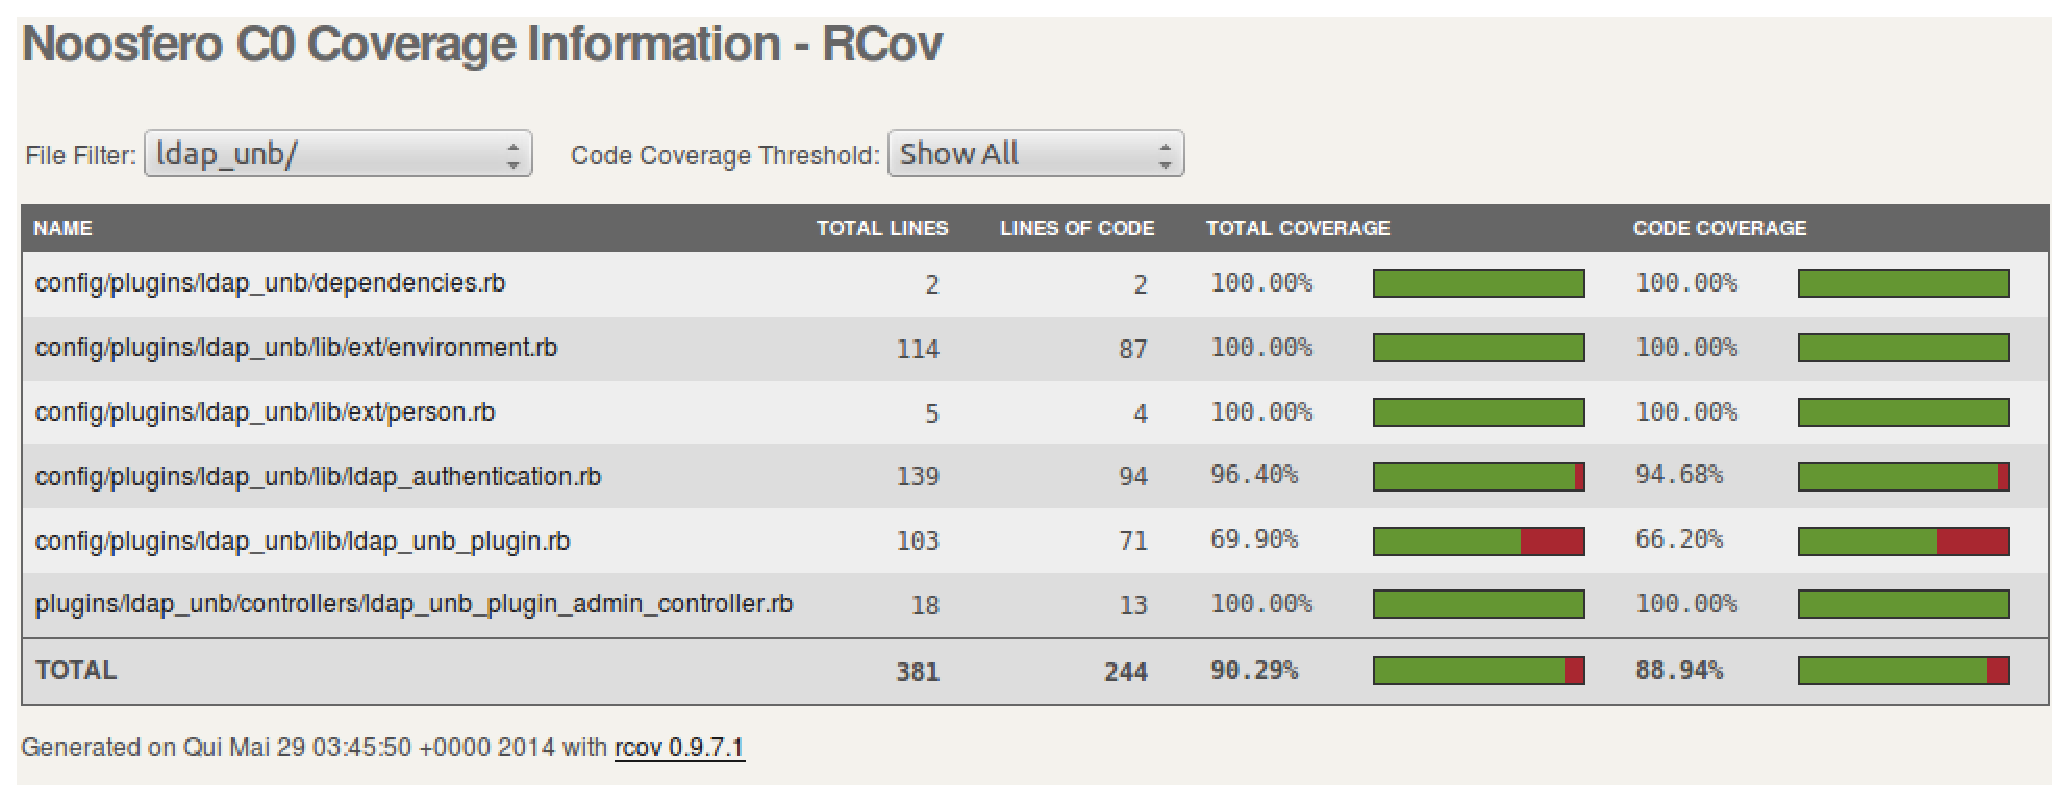
\includegraphics[keepaspectratio=false,scale=0.45]
      {figuras/cobertura_teste.eps}
    \caption{Cobertura de código do plugin LdapUnb}
    \label{consideracoes_cobertura1}
\end{figure}


Não desenvolvemos testes de aceitação para o \textit{plugin} LDAP UnB, pelo fato de ser uma aplicação que opera a maior parte das suas funcionalidades nas camadas mais baixas do sistema, alterando muito pouco a percepção do usuário.

\subsection{Plugin para envio de TCC}

Este \textit{plugin} também foi desenvolvido para a plataforma Noosfero, porém em uma aplicação diferente, o Portal UnB Gama. A ideia deste \textit{plugin} surgiu da necessidade de existir um ambiente virtual em que os trabalhos de conclusão de curso pudessem ser submetidos aos professores e compartilhados com a comunidade acadêmica, buscando assim manter uma forma de versionamento dos trabalhos desenvolvidos e dispensando a necessidade de trabalhos de conclusão de curso impressos.
%
Este \textit{plugin} é responsável por criar uma atribuição de trabalhos, chamada de \textit{work assignment}. Essa atribuição possui algumas funcionalidades específicas como possibilitar que os usuários envolvidos sejam notificados via \textit{email} sobre a submissão de um certo trabalho. Para tal foi necessário instanciar um servidor de \textit{email} para executar estas notificações, assim como criar uma página no Portal FGA\footnote{url{fga.unb.br}} para que o usuário pudesse submeter seu trabalho.
%
Para validar o desenvolvimento desta funcionalidade desenvolvemos os seguintes tipos de testes: funcionais, unitário e de aceitação. Abaixo encontra-se descrita a história de usuário referente \textit{plugin} para envio de TCC:
\begin{enumerate}
\item  \textbf{Plugin para envio de TCC}

\textbf{Como} usuário

\textbf{Gostaria} de submeter um trabalho para uma comunidade, seguindo um formulário (título, nome do remetente, \textit{email} do destinatário, nome do destinatário e descrição) enviando um aviso para ambas as partes

\textbf{para} manter um versionamento do trabalho.


\textbf{Cenário:}

\textbf{Dado} que estou autenticado como ``usuário''

\textbf{Quando} eu entrar no painel de controle da ``Minha Comunidade''

\textbf{E} entrar em ``Gerenciar Conteúdo''

\textbf{E} entrar em ``Novo Conteúdo''

\textbf{E} entrar em ``Trabalho a ser entregue''

\textbf{E} preencher o campo ``Título''

\textbf{E} clicar em ``Salvar''

\textbf{Então} eu devo ser redirecionado à pagina de ``Gerenciar Conteúdos''

\textbf{E} visualizar o campo ``Título''

\textbf{Quando} eu entrar em ``Carregar Arquivo''

\textbf{E} marcar o campo ``Enviar notificação''

\textbf{E} preencher o campo ``Assunto''

\textbf{E} preencher o campo ``Destinatário''

\textbf{E} clicar em ``Enviar''

\textbf{Então} eu devo visualizar ``Enviando com sucesso''

\end{enumerate}

Os testes funcionais do \textit{plugin} para envio de TCC são responsáveis por verificar os seguintes fatores:

\begin{itemize}
\item Permissão para enviar trabalhos somente para usuários autorizados;
\item Capacidade de enviar um arquivo ou mais;
\item Capacidade de atualizar um arquivo enviado;
\item Validação de arquivos;
\item Capacidade de enviar \textit{email} aos usuários envolvidos;
\item Tratamento do redirecionamento das páginas;
\item Capacidade de deletar arquivos por usuários autorizados;
\item Capacidade de carregar arquivos por usuários envolvidos;
\end{itemize}

Os testes unitários deste \textit{plugin} são responsáveis por verificar os seguintes parâmetros:

\begin{itemize}
\item Nome do \textit{plugin};
\item Descrição do \textit{plugin};
\item Possibilidade de submissão de um arquivo por um usuário;
\item Nome do arquivo;
\item Versão do arquivo;
\item Autor do arquivo;
\end{itemize}

A ferramenta Rcov também foi utilizada para dimensionar a taxa de cobertura de código do \textit{plugin} para envio de TCC, segue os dados sobre a execução dos testes funcionais e unitários:

\begin{itemize}
\item Quantidade de testes executados: \textbf{28 testes};
\item Quantidade de assertivas executadas: \textbf{84 assertivas};
\item Quantiadde de falhas obtidas: \textbf{0 falhas};
\item Tempo de execução dos testes: \textbf{10,5 segundos};
\end{itemize}

Na imagem \ref{consideracoes_cobertura2} está representado a cobertura de código, extraída da ferramenta Rcov:

\begin{figure}[!h]
    \centering
    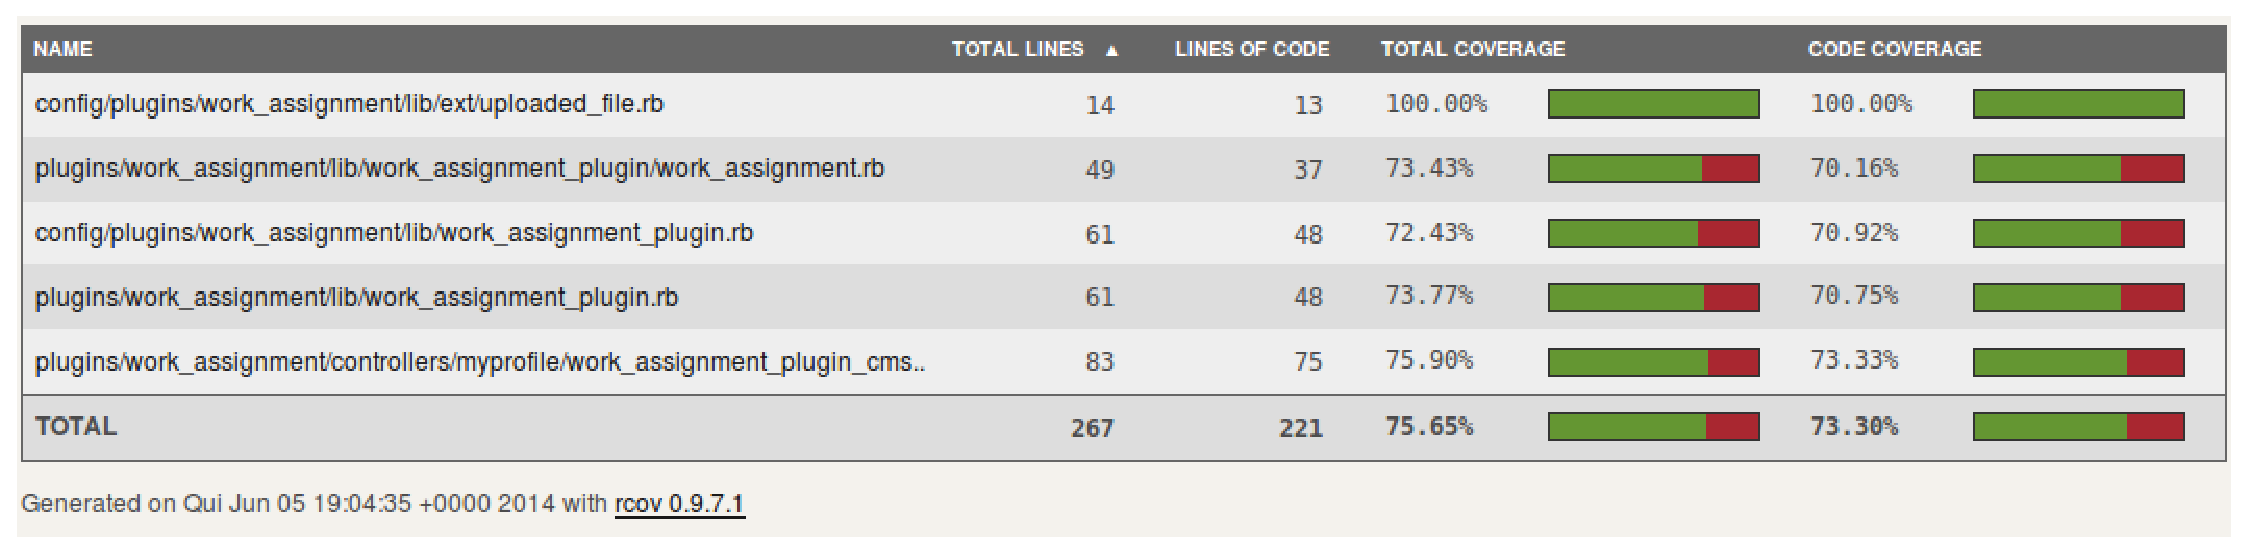
\includegraphics[keepaspectratio=false,scale=0.45]
      {figuras/cobertura_tcc.eps}
    \caption{Cobertura de código do plugin para submissão de trabalho}
    \label{consideracoes_cobertura2}
\end{figure}

Por fim, os testes de aceitação do \textit{plugin} para envio de TCC são responsáveis por verificar os seguintes fatores:

\begin{itemize}
\item Capacidade de criar, editar e deletar uma atribuição de trabalhos (\textit{work assignment});
\item Validação de parâmetros durante a criação e edição de uma atribuição de trabalhos;
\item Capacidade de enviar e receber \textit{emails} sobre o envio de um trabalho;
\item Capacidade de postar comentários sobre uma atribuição de trabalhos;
\item Capacidade de reportar problemas;
\end{itemize}

Abaixo está descrito um exemplo de teste desenvolvido para o \textit{plugin} (os demais testes estão descritos no apêndice B):
%Done: deixar um cenário de exemplo e colocar os demais em um Apêndice

\textbf{Feature: send work plugin}

\textbf{As} an user

\textbf{I want} to send work with notification email

\textbf{Background:}

\textbf{Given} ``Work Assignment'' plugin is enabled

\textbf{Given} the following users

      | login     | name          |

      | joaosilva | Joao da Silva |

      | josesilva | Jose da Silva |

\textbf{And} the following community

      | identifier  | name         |

      | mycommunity | My Community |

\textbf{And} ``Joao da Silva" is admin of ``My Community"

\textbf{And} I am logged in as admin

\textbf{And} I go to /admin/plugins

\textbf{And} I check ``Work Assignment"

\textbf{And} I press ``Save changes"

\textbf{Then} I should see ``Plugins updated successfully." 


\begin{enumerate}
\item  \textbf{Scenario:} Upload a file to work assignment and send a email
    
    \textbf{Given} I am logged in as ``joaosilva" 
    
    \textbf{When} I follow ``My Community"
    
    \textbf{When} I go to mycommunity's control panel
    
    \textbf{And} I follow ``Manage Content"
    
    \textbf{And} I follow ``New content"
    
    \textbf{And} I follow ``Work Assignment"
    
    \textbf{Then} I should be on /myprofile/mycommunity/cms/new
    
    \textbf{When} I fill in ``Title" with ``test"
    
    \textbf{And} I press ``Save"
    
    \textbf{Then} I should be on /mycommunity/test
    
    \textbf{When} I follow ``Upload files"
    
    \textbf{And} I check ``Send notification"
    
    \textbf{And} I attach the file ``public/images/rails.png" to ``uploadedfiles"
    
    \textbf{And} I press ``Upload"
    
    \textbf{Then} I should be on /myprofile/mycommunity/cms/sendemail
    
    \textbf{When} I fill in ``Title" with ``Work"
    
    \textbf{And} I fill in ``Receiver" with ``josesilva@example.com"
    
    \textbf{And} I fill in ``Message" with ``test"
    
    \textbf{And} I press ``Send"
    
    \textbf{Then} I should see ``Contact sent successfully"

Após a execução dos testes desenvolvidos, obtivemos os seguintes dados:

\begin{itemize}
\item Quantidade de cenários executados: \textbf{6 cenários};
\item Quantidade de passos executadas: \textbf{130 passos};
\item Quantiadde de falhas obtidas: \textbf{0 falhas};
\item Tempo de execução dos testes: \textbf{7 minutos e 18 segundos};
\end{itemize}

\subsection{Observações obtidas}

O \textit{plugin} LDAP UnB encontra-se ainda em fase de testes na rede Comunidade.UnB. 
%
O \textit{plugin} para envio de TCC também encontra-se em fase de testes, com um piloto já disponível para utilização pelos alunos de graduação do curso de engenharia de software da FGA.

A partir da cobertura dos testes do \textit{plugin} de envio de TCC, foi verificado que existe uma necessidade de refatoração desta funcionalidade, considerando alguns aspectos que dificultaram o desenvolvimento de testes desta funcionalidade, como a duplicação de código.
%
Porém estes resultados preliminares foram considerados satisfatórios, considerando que outros \textit{plugins} desenvolvidos pela comunidade do Noosfero e já homologados apresentam métricas semelhantes.

\begin{itemize}
\item Plugin Stoa: \textit{Plugin} que inclui funcionalidades ao Stoa, rede colaborativa da USP (Universidade de São Paulo)

\begin{figure}[!h]
    \centering
    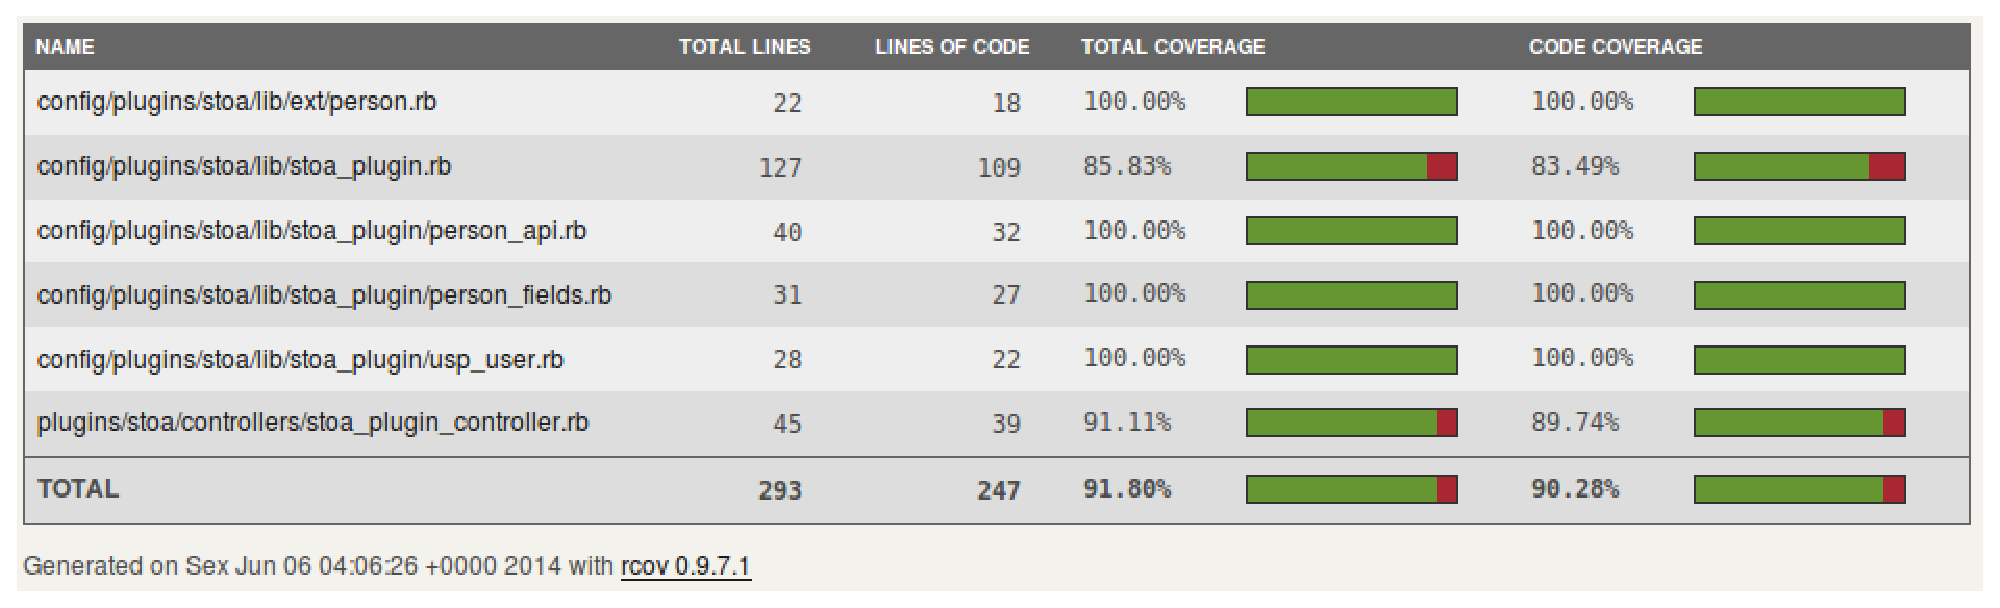
\includegraphics[keepaspectratio=false,scale=0.45]
      {figuras/stoa.eps}
    \caption{Cobertura de código do plugin Stoa}
    \label{consideracoes_cobertura3}
\end{figure}

\item Plugin Ldap: \textit{Plugin} que permite autenticação via Ldap;

\begin{figure}[!h]
    \centering
    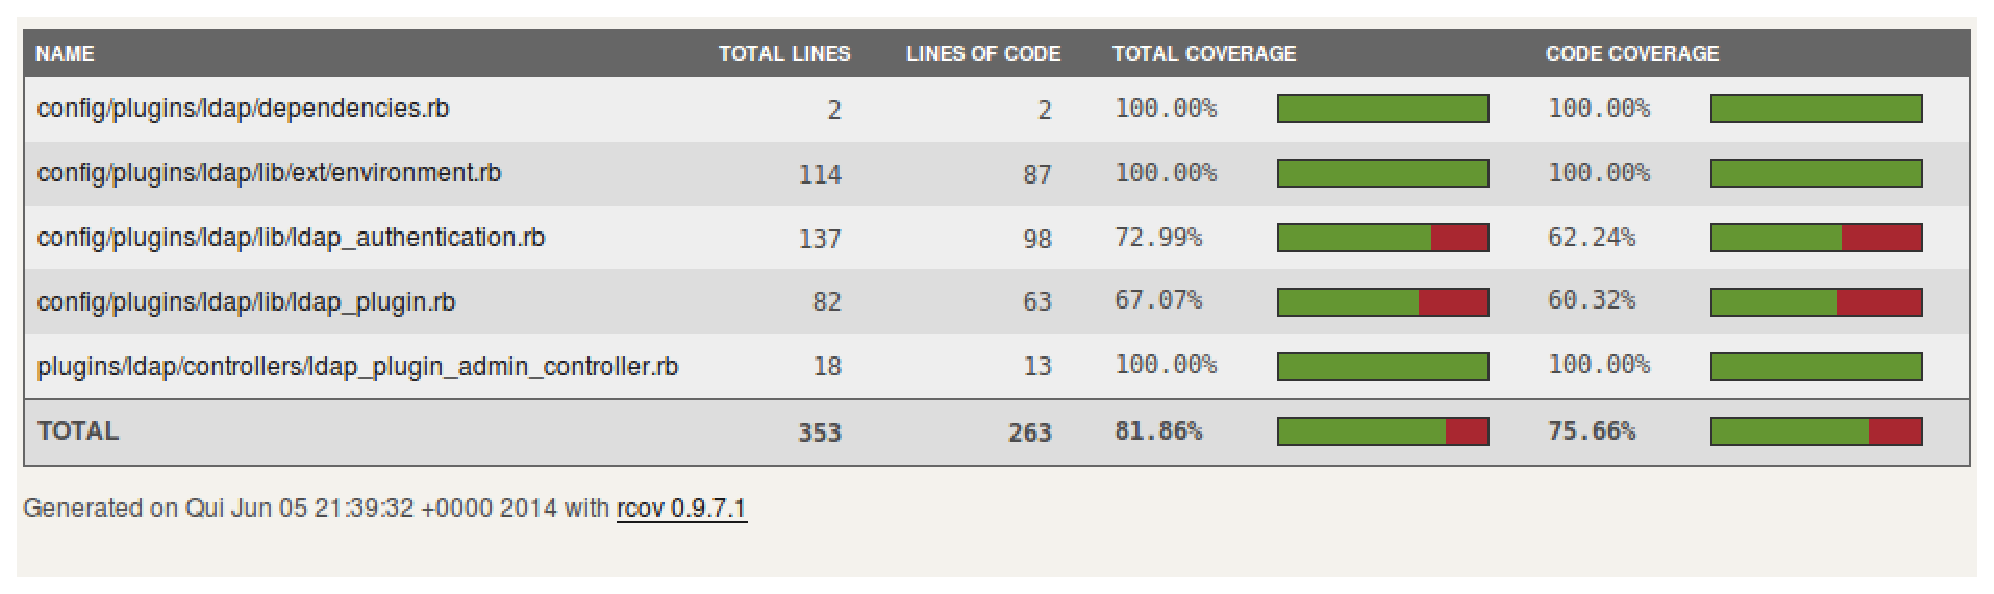
\includegraphics[keepaspectratio=false,scale=0.45]
      {figuras/ldap.eps}
    \caption{Cobertura de código do plugin Ldap}
    \label{consideracoes_cobertura4}
\end{figure}

\item plugin Statistics: \textit{Plugin} que permite adicionar um bloco de estatísticas ao perfil do usuário

\begin{figure}[!h]
    \centering
    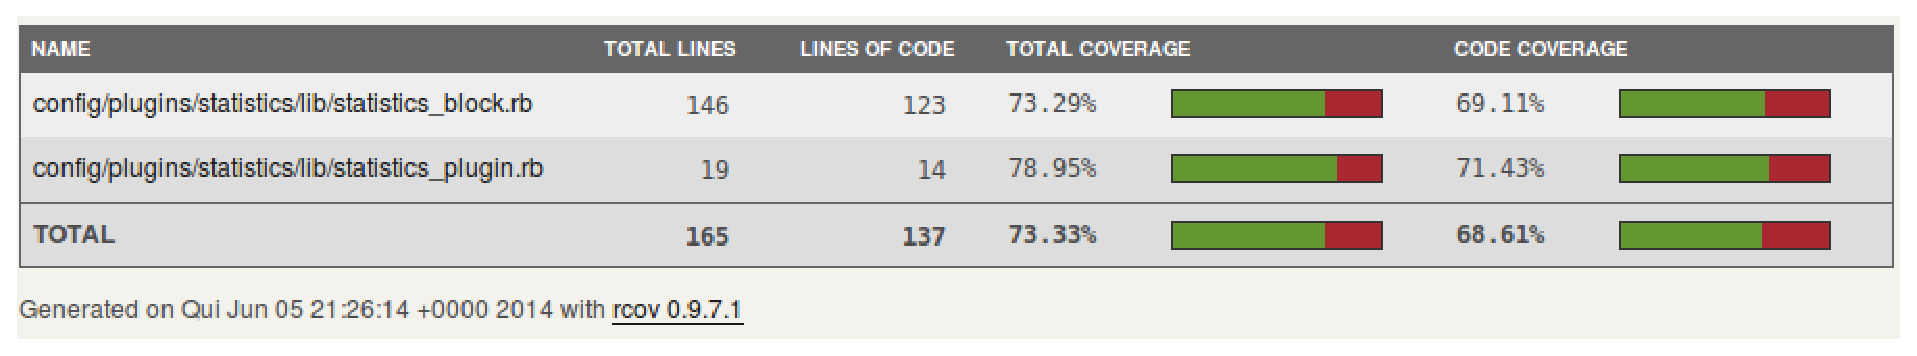
\includegraphics[keepaspectratio=false,scale=0.45]
      {figuras/statistics.eps}
    \caption{Cobertura de código do plugin Statistics}
    \label{consideracoes_cobertura3}
\end{figure}

\end{itemize}


\section{Considerações finais}

O desenvolvimento de testes automatizados é uma prática constante no desenvolvimento da plataforma noosfero e importante na validação de novos recursos desenvolvidos. Assim conseguimos verificar que a utilização de práticas de TDD e BDD como base para o desenvolvimento trouxe resultados satisfatórios, como será mostrado no capítulo a seguir.

Com a proposta de algumas técnicas de avaliação da usabilidade para o Portal da Participação Social, verificamos que muitas delas precisam ser adaptadas para uma melhor adoção nos ambientes de software livre e em métodos ágeis. O teste de usabilidade proposto foi planejado pensando nas práticas clássicas de avaliação da usabilidade que é considerada por vários autores como uma das melhores maneiras de avaliar uma interface.





